% Options for packages loaded elsewhere
\PassOptionsToPackage{unicode}{hyperref}
\PassOptionsToPackage{hyphens}{url}
\PassOptionsToPackage{dvipsnames,svgnames,x11names}{xcolor}
\documentclass[
  brazilian,
  12pt,
]{article}
\usepackage{xcolor}
\usepackage[margin=2.5cm]{geometry}
\usepackage{amsmath,amssymb}
\setcounter{secnumdepth}{-\maxdimen} % remove section numbering
\usepackage{iftex}
\ifPDFTeX
  \usepackage[T1]{fontenc}
  \usepackage[utf8]{inputenc}
  \usepackage{textcomp} % provide euro and other symbols
\else % if luatex or xetex
  \usepackage{unicode-math} % this also loads fontspec
  \defaultfontfeatures{Scale=MatchLowercase}
  \defaultfontfeatures[\rmfamily]{Ligatures=TeX,Scale=1}
\fi
\usepackage{lmodern}
\ifPDFTeX\else
  % xetex/luatex font selection
\fi
% Use upquote if available, for straight quotes in verbatim environments
\IfFileExists{upquote.sty}{\usepackage{upquote}}{}
\IfFileExists{microtype.sty}{% use microtype if available
  \usepackage[]{microtype}
  \UseMicrotypeSet[protrusion]{basicmath} % disable protrusion for tt fonts
}{}
\makeatletter
\@ifundefined{KOMAClassName}{% if non-KOMA class
  \IfFileExists{parskip.sty}{%
    \usepackage{parskip}
  }{% else
    \setlength{\parindent}{0pt}
    \setlength{\parskip}{6pt plus 2pt minus 1pt}}
}{% if KOMA class
  \KOMAoptions{parskip=half}}
\makeatother
\usepackage{longtable,booktabs,array}
\newcounter{none} % for unnumbered tables
\usepackage{calc} % for calculating minipage widths
% Correct order of tables after \paragraph or \subparagraph
\usepackage{etoolbox}
\makeatletter
\patchcmd\longtable{\par}{\if@noskipsec\mbox{}\fi\par}{}{}
\makeatother
% Allow footnotes in longtable head/foot
\IfFileExists{footnotehyper.sty}{\usepackage{footnotehyper}}{\usepackage{footnote}}
\makesavenoteenv{longtable}
\usepackage{graphicx}
\makeatletter
\newsavebox\pandoc@box
\newcommand*\pandocbounded[1]{% scales image to fit in text height/width
  \sbox\pandoc@box{#1}%
  \Gscale@div\@tempa{\textheight}{\dimexpr\ht\pandoc@box+\dp\pandoc@box\relax}%
  \Gscale@div\@tempb{\linewidth}{\wd\pandoc@box}%
  \ifdim\@tempb\p@<\@tempa\p@\let\@tempa\@tempb\fi% select the smaller of both
  \ifdim\@tempa\p@<\p@\scalebox{\@tempa}{\usebox\pandoc@box}%
  \else\usebox{\pandoc@box}%
  \fi%
}
% Set default figure placement to htbp
\def\fps@figure{htbp}
\makeatother
\ifLuaTeX
\usepackage[bidi=basic,shorthands=off]{babel}
\else
\usepackage[bidi=default,shorthands=off]{babel}
\fi
\ifLuaTeX
  \usepackage{selnolig} % disable illegal ligatures
\fi
\setlength{\emergencystretch}{3em} % prevent overfull lines
\providecommand{\tightlist}{%
  \setlength{\itemsep}{0pt}\setlength{\parskip}{0pt}}
\usepackage{bookmark}
\IfFileExists{xurl.sty}{\usepackage{xurl}}{} % add URL line breaks if available
\urlstyle{same}
\hypersetup{
  pdftitle={Planejamento Agregado da Produção sob Demanda Sazonal e Incerta: uma Decisão Integrada de Produção{,} Força de Trabalho e Estoque},
  pdfauthor={Tiago André Gondim --- Matrícula 231013476; Universidade de Brasília --- FT --- Engenharia de Produção; Prof.~João Gabriel de Moraes Souza},
  pdflang={pt-BR},
  colorlinks=true,
  linkcolor={Maroon},
  filecolor={Maroon},
  citecolor={Blue},
  urlcolor={Blue},
  pdfcreator={LaTeX via pandoc}}

\title{Planejamento Agregado da Produção sob Demanda Sazonal e Incerta:
uma Decisão Integrada de Produção, Força de Trabalho e Estoque}
\author{Tiago André Gondim --- Matrícula 231013476 \and Universidade de
Brasília --- FT --- Engenharia de Produção \and Prof.~João Gabriel de
Moraes Souza}
\date{Brasília, 2026}

\begin{document}
\maketitle

\subsection{1. Resumo executivo}\label{resumo-executivo}

Neste projeto formulo e resolvo o problema de \textbf{planejamento
agregado da produção} de um fabricante de ventiladores domésticos com
demanda fortemente sazonal, decidindo, para um horizonte de 12 meses,
\textbf{quanto produzir} (em tempo regular e em hora extra),
\textbf{qual o tamanho da força de trabalho} (contratações e demissões)
e \textbf{quanto manter em estoque} em cada mês, ao menor custo total,
respeitando a capacidade e um nível de serviço-alvo.

O método integra três frentes da disciplina: (i) \textbf{previsão de
demanda} com modelos de séries temporais, validada em backtest, que gera
a demanda a planejar e a distribuição do erro; (ii) \textbf{programação
linear} de custo-relevante, que produz o plano ótimo e permite comparar
estratégias e extrair preços-sombra; e (iii) \textbf{gestão de estoque e
nível de serviço}, em que o erro de previsão dimensiona o estoque de
segurança e uma simulação de Monte Carlo mede a robustez do plano.

O principal resultado é que o \textbf{plano misto} (que combina
antecipação em estoque, ajuste moderado da força de trabalho e hora
extra no pico) custa \textbf{R\$ 4,92 milhões} e domina as duas
estratégias puras: a de \textbf{nível} custa 5,2\% a mais (excesso de
estoque) e a de \textbf{perseguição} 15,2\% a mais
(contratações/demissões e atrasos no pico). A decisão recomendada é
\textbf{adotar o plano misto com estoque de segurança calibrado para
95\% de nível de serviço}, que eleva o serviço realizado sob incerteza e
protege contra os cenários adversos a um acréscimo de custo de cerca de
2\%.

\begin{center}\rule{0.5\linewidth}{0.5pt}\end{center}

\subsection{2. Contexto e formulação do
problema}\label{contexto-e-formulauxe7uxe3o-do-problema}

\subsubsection{2.1 Sistema produtivo}\label{sistema-produtivo}

Considero uma fábrica brasileira de ventiladores domésticos de pequeno
porte, cujo portfólio é agregado em um produto equivalente (uma prática
usual em planejamento agregado, em que se planeja por família e não por
SKU). A produção é \emph{make-to-stock}: é possível produzir
antecipadamente e estocar. A demanda tem forte sazonalidade de verão.
Adoto um ano de planejamento que começa na baixa estação (mês 1), sobe
até o pico no mês 7 e retorna à baixa ao final do horizonte.

\subsubsection{2.2 O problema como decisão de
PCP}\label{o-problema-como-decisuxe3o-de-pcp}

O trabalho não descreve uma empresa: ele resolve uma \textbf{decisão}.
Formalmente, para cada mês \(t = 1,\dots,12\) preciso decidir
simultaneamente:

\begin{itemize}
\tightlist
\item
  \(P_t\): produção em tempo regular (un);
\item
  \(O_t\): produção em hora extra (un);
\item
  \(W_t\): número de trabalhadores;
\item
  \(H_t, F_t\): contratações e demissões;
\item
  \(I_t\): estoque ao fim do mês;
\item
  \(B_t\): demanda atendida com atraso (backorder).
\end{itemize}

O objetivo é minimizar o \textbf{custo total relevante} do plano,
sujeito às restrições operacionais descritas na Seção 4.

\subsubsection{2.3 Hipóteses}\label{hipuxf3teses}

\begin{itemize}
\tightlist
\item
  Um único produto agregado; demanda mensal ao longo de 12 meses.
\item
  Custos determinísticos e conhecidos; a incerteza está na demanda,
  tratada via erro de previsão.
\item
  A produção regular é limitada pela força de trabalho
  (\(P_t \le k\,W_t\), com \(k = 180\) un/trabalhador/mês); a hora extra
  é limitada a uma fração da capacidade regular.
\item
  O custo de material por unidade é aproximadamente constante (a
  produção anual é próxima da demanda anual) e, por isso, é excluído da
  função-objetivo, prática padrão em planejamento agregado. Os custos
  que efetivamente movem a decisão são salário, hora extra, estoque,
  contratação, demissão e atraso.
\end{itemize}

\subsubsection{2.4 Restrições operacionais e
indicadores}\label{restriuxe7uxf5es-operacionais-e-indicadores}

As restrições completas estão na Seção 4. Os \textbf{indicadores de
desempenho} que acompanho são: custo total relevante, nível de serviço
(fill rate), estoque médio e de pico, utilização da capacidade,
rotatividade da força de trabalho (contratações + demissões) e volume de
atrasos.

A Tabela 1 resume as premissas do caso.

\textbf{Tabela 1 - Premissas do caso}

{\def\LTcaptype{none} % do not increment counter
\begin{longtable}[]{@{}lll@{}}
\toprule\noalign{}
Grupo & Parâmetro & Valor \\
\midrule\noalign{}
\endhead
\bottomrule\noalign{}
\endlastfoot
Demanda & Nível médio & 17.000 un/mês \\
& Amplitude sazonal & ±46\% \\
& Mês de pico & 7 \\
& Tendência & +6\% ao ano \\
& CV do erro de previsão & 8\% \\
Capacidade & Produtividade & 180 un/trab/mês \\
& Trabalhadores iniciais & 88 \\
& Estoque inicial & 2.000 un \\
& Teto de hora extra & 12\% da cap. regular \\
& Ajuste de mão de obra & ±4 trab/mês \\
Custos (BRL) & Salário & 3.500 /trab/mês \\
& Hora extra & 30 /un \\
& Estoque & 6 /un/mês \\
& Contratação & 2.500 /trab \\
& Demissão & 5.000 /trab \\
& Atraso & 50 /un/mês \\
Serviço & Nível-alvo & 95\% (z = 1,645) \\
\end{longtable}
}

A capacidade regular inicial é de 15.840 un/mês (17.741 un/mês com hora
extra máxima). Como o pico de demanda chega a 25.565 un, \textbf{nem
mesmo a capacidade com hora extra da força inicial atende o pico}:
atravessá-lo exige antecipar produção em estoque na baixa estação e/ou
ampliar a força de trabalho ao longo dos meses anteriores. Essa é a
tensão central do problema.

\begin{center}\rule{0.5\linewidth}{0.5pt}\end{center}

\subsection{3. Dados e preparação}\label{dados-e-preparauxe7uxe3o}

Optei por \textbf{dados simulados}, escolha permitida pelo enunciado e
adequada ao objetivo, que é analisar cenários controlados, variabilidade
e políticas alternativas. A simulação me permite conhecer o processo
gerador e, assim, avaliar de forma limpa o erro de previsão e a robustez
das decisões.

A demanda esperada segue um sinal sazonal com tendência:

\[D(t) = 17000 \cdot \left(1 + 0{,}46\,\sin\!\left(\tfrac{2\pi (t-7)}{12} + \tfrac{\pi}{2}\right)\right)\cdot\left(1 + 0{,}06\,\tfrac{t-1}{12}\right).\]

A demanda observada acrescenta ruído multiplicativo
\(\varepsilon_t \sim \mathcal{N}(0,\,0{,}08^2)\). Para a etapa de
previsão, gero 5 anos de histórico mensal consistentes com essa demanda
e com a tendência anual, de modo que os modelos possam ser ajustados e
validados antes de projetar o ano de planejamento. Toda a aleatoriedade
usa uma semente fixa, garantindo reprodutibilidade (Seção 5). A Figura 1
mostra a demanda do ano de planejamento e a linha de capacidade regular
inicial, evidenciando os sete meses em que a demanda supera a capacidade
regular.

\begin{figure}
\centering
\pandocbounded{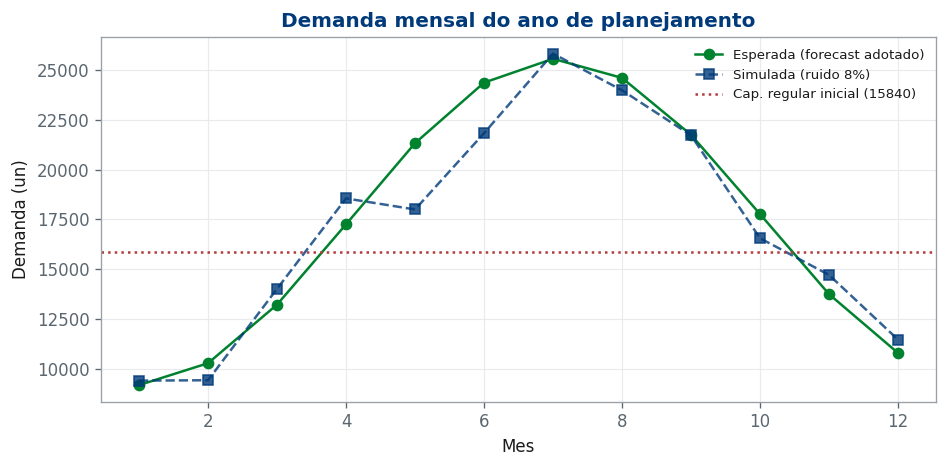
\includegraphics[keepaspectratio,alt={Figura 1 - Demanda mensal do ano de planejamento.}]{figuras/fig01_demanda.png}}
\caption{Figura 1 - Demanda mensal do ano de planejamento.}
\end{figure}

\begin{center}\rule{0.5\linewidth}{0.5pt}\end{center}

\subsection{4. Modelagem quantitativa}\label{modelagem-quantitativa}

\subsubsection{4.1 Previsão de demanda}\label{previsuxe3o-de-demanda}

Comparo quatro modelos, alinhados ao ferramental da disciplina
(\texttt{statsmodels}, \texttt{scikit-learn}): dois baselines sem
sazonalidade --- \textbf{média móvel} e \textbf{suavização exponencial
simples (SES)} --- e dois modelos sazonais --- \textbf{Holt-Winters}
(tendência aditiva, sazonalidade multiplicativa, período 12) e
\textbf{SARIMA} \((1,1,1)\times(1,1,0)_{12}\). O ajuste é feito no
histórico e a avaliação em um \emph{holdout} de 12 meses (um ciclo
sazonal completo), medindo MAE, RMSE e MAPE. O modelo escolhido é
reajustado no histórico completo para projetar o ano de planejamento, e
o erro do backtest fornece a distribuição usada no estoque de segurança
e no Monte Carlo.

\subsubsection{4.2 Planejamento agregado (programação
linear)}\label{planejamento-agregado-programauxe7uxe3o-linear}

A função-objetivo minimiza o custo total relevante:

\[\min \; Z = \sum_{t=1}^{12} \Big( c_W W_t + c_O O_t + c_I I_t + c_H H_t + c_F F_t + c_B B_t \Big),\]

com \(c_W\) salário, \(c_O\) hora extra, \(c_I\) estoque, \(c_H\)
contratação, \(c_F\) demissão e \(c_B\) atraso. Sujeito a, para cada mês
\(t\):

\[
\begin{aligned}
& I_t - B_t = I_{t-1} - B_{t-1} + P_t + O_t - D_t && \text{(balanço de estoque)}\\
& W_t = W_{t-1} + H_t - F_t && \text{(balanço de força de trabalho)}\\
& P_t \le k\,W_t && \text{(capacidade regular)}\\
& O_t \le \theta\,k\,W_t && \text{(teto de hora extra)}\\
& H_t \le H^{\max}, \quad F_t \le F^{\max} && \text{(limites de ajuste)}\\
& B_{12} = 0 && \text{(atender toda a demanda)}\\
& P_t, O_t, W_t, H_t, F_t, I_t, B_t \ge 0.
\end{aligned}
\]

A produção regular não tem custo unitário adicional na função-objetivo
porque o custo da mão de obra já está no salário \(c_W W_t\), pago
independentemente da produção. Essa é a escolha de modelagem que
preserva o trade-off clássico do planejamento agregado: manter uma força
de trabalho grande custa salário todo mês, o que dá valor a demiti-la na
baixa estação.

\subsubsection{4.3 Estratégias e análise de
sensibilidade}\label{estratuxe9gias-e-anuxe1lise-de-sensibilidade}

As três estratégias canônicas são o mesmo PL com restrições adicionais:
\textbf{nível} impõe força de trabalho constante (\(W_t = W_1\));
\textbf{perseguição} impõe estoque de antecipação nulo (\(I_t = 0\));
\textbf{mista} deixa todos os instrumentos livres. Para a fronteira
custo × serviço, adiciono a restrição de estoque de segurança
\(I_t \ge z\cdot \mathrm{CV}_{\text{erro}}\cdot D_t\), variando \(z\)
conforme o nível de serviço.

\begin{center}\rule{0.5\linewidth}{0.5pt}\end{center}

\subsection{5. Implementação
computacional}\label{implementauxe7uxe3o-computacional}

O projeto é implementado em Python 3.13, com
\texttt{numpy}/\texttt{pandas} (dados), \texttt{statsmodels} e
\texttt{scikit-learn} (previsão), \texttt{PuLP} com o solver CBC
(programação linear), \texttt{matplotlib} (gráficos) e \texttt{scipy}
(distribuições). A organização separa responsabilidades: os parâmetros
do caso ficam em um único módulo (\texttt{src/parametros.py}), o modelo
de PL em \texttt{src/modelo.py} (fonte única, reutilizada pelo notebook
e pelas verificações), e o notebook
\texttt{notebooks/projeto\_pcp.ipynb} conduz a análise ponta a ponta.

A \textbf{reprodutibilidade} é assegurada por: semente global única,
dependências com versões fixadas (\texttt{requirements.txt}), dados
gerados salvos em disco e notebook exportado em HTML. Antes de construir
a análise, verifiquei que o caso é \textbf{não-trivial} por um script
independente (\texttt{src/valida\_premissas.py}): resolvendo os três
planos como PLs, confirmei que o plano misto vence as estratégias puras
e que a capacidade é efetivamente estressada pela sazonalidade ---
evitando o risco de calibrar um problema em que uma estratégia simples
já fosse ótima. Em conformidade com o enunciado, o código não é colado
neste PDF; está no repositório público e no notebook (que o GitHub
renderiza com os resultados).

\begin{center}\rule{0.5\linewidth}{0.5pt}\end{center}

\subsection{6. Resultados e análise de
cenários}\label{resultados-e-anuxe1lise-de-cenuxe1rios}

\subsubsection{6.1 Previsão de demanda}\label{previsuxe3o-de-demanda-1}

A Tabela 2 e a Figura 2 mostram o desempenho no holdout. Os modelos
sazonais dominam com folga: o \textbf{SARIMA} obtém MAPE de 5,4\% e o
Holt-Winters 6,4\%, contra 28,9\% da média móvel e 34,8\% da SES. O
resultado ilustra a lição de que baselines sem estrutura sazonal são
inadequados para demanda sazonal. Escolho o SARIMA. O erro do modelo no
holdout equivale a cerca de \textbf{8\% da demanda média} --- coerente
com o ruído do processo gerador, o que valida o pipeline ---, e é esse
coeficiente de variação que dimensiona o estoque de segurança: no pico,
o estoque de segurança para 95\% de serviço é de aproximadamente 3.373
un.

\textbf{Tabela 2 - Erro de previsão no holdout (12 meses)}

{\def\LTcaptype{none} % do not increment counter
\begin{longtable}[]{@{}llll@{}}
\toprule\noalign{}
Modelo & MAE (un) & RMSE (un) & MAPE (\%) \\
\midrule\noalign{}
\endhead
\bottomrule\noalign{}
\endlastfoot
SARIMA & 888 & 1.310 & 5,4 \\
Holt-Winters & 1.119 & 1.526 & 6,4 \\
Média Móvel(3) & 5.058 & 5.978 & 28,9 \\
SES & 6.671 & 8.217 & 34,8 \\
\end{longtable}
}

\begin{figure}
\centering
\pandocbounded{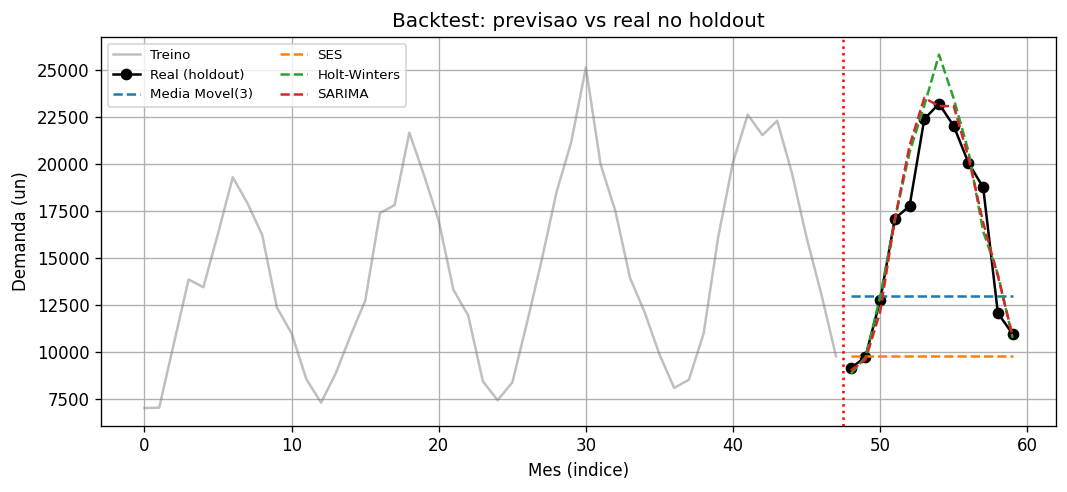
\includegraphics[keepaspectratio,alt={Figura 2 - Backtest: previsão vs real no holdout.}]{figuras/fig02_backtest.png}}
\caption{Figura 2 - Backtest: previsão vs real no holdout.}
\end{figure}

\subsubsection{6.2 O plano agregado misto}\label{o-plano-agregado-misto}

A Figura 3 mostra o plano ótimo. A leitura operacional é nítida: nos
meses de baixa (1 a 4) a fábrica \textbf{produz acima da demanda e
acumula estoque} (que chega a \textasciitilde15.700 un no mês 4); a
força de trabalho \textbf{cresce gradualmente de 88 para 104}
trabalhadores rumo ao pico; e a \textbf{hora extra é acionada apenas nos
meses 6 a 9}, o núcleo da alta estação. Não há atrasos. Ou seja, o plano
atravessa o pico com uma combinação de estoque antecipado, força de
trabalho ampliada e hora extra pontual --- exatamente o que a intuição
de PCP recomenda, aqui quantificado.

\begin{figure}
\centering
\pandocbounded{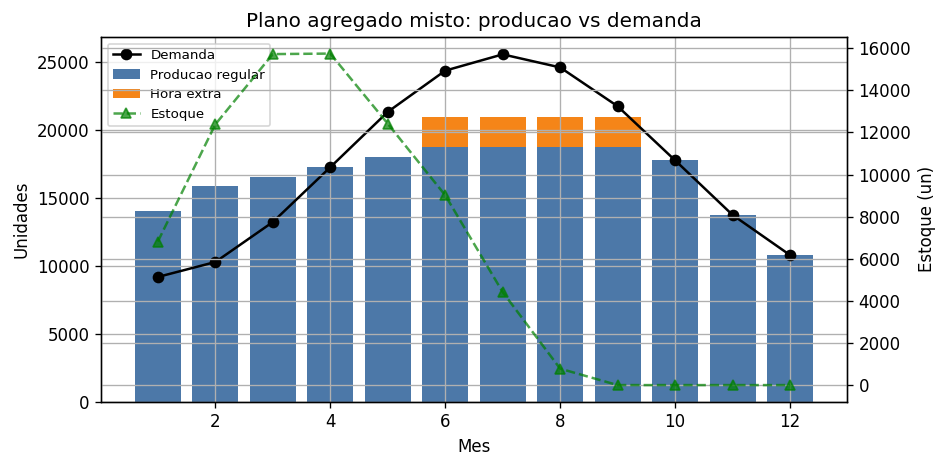
\includegraphics[keepaspectratio,alt={Figura 3 - Plano agregado misto: produção vs demanda, com estoque.}]{figuras/fig03_plano_misto.png}}
\caption{Figura 3 - Plano agregado misto: produção vs demanda, com
estoque.}
\end{figure}

\subsubsection{6.3 Comparação de
estratégias}\label{comparauxe7uxe3o-de-estratuxe9gias}

A Tabela 3 e as Figuras 4 e 5 comparam as três estratégias. O custo do
plano misto é \textbf{R\$ 4.915.334}. As estratégias puras são mais
caras e falham por motivos distintos:

\begin{itemize}
\tightlist
\item
  A \textbf{estratégia de nível} (força de trabalho constante em 92
  trabalhadores) evita a rotatividade de mão de obra, mas para
  atravessar o pico com produção mais estável precisa \textbf{acumular
  muito mais estoque} (pico de \textasciitilde24.900 un) e recorrer a
  mais hora extra; custa \textbf{5,2\% a mais} (R\$ 255 mil), sobretudo
  em estoque.
\item
  A \textbf{estratégia de perseguição} (sem estoque de antecipação) zera
  o estoque ocioso, mas precisa \textbf{ajustar a força de trabalho
  intensamente} e, como os limites de ±4 trabalhadores/mês impedem
  acompanhar o salto sazonal, acaba \textbf{atrasando demanda no pico};
  custa \textbf{15,2\% a mais} (R\$ 746 mil), em contratações, demissões
  e atrasos.
\end{itemize}

\textbf{Tabela 3 - Custo por estratégia (R\$)}

{\def\LTcaptype{none} % do not increment counter
\begin{longtable}[]{@{}lll@{}}
\toprule\noalign{}
Estratégia & Custo total & Diferença vs misto \\
\midrule\noalign{}
\endhead
\bottomrule\noalign{}
\endlastfoot
Misto & 4.915.334 & --- \\
Nível & 5.170.426 & +5,2\% \\
Perseguição & 5.661.200 & +15,2\% \\
\end{longtable}
}

\begin{figure}
\centering
\pandocbounded{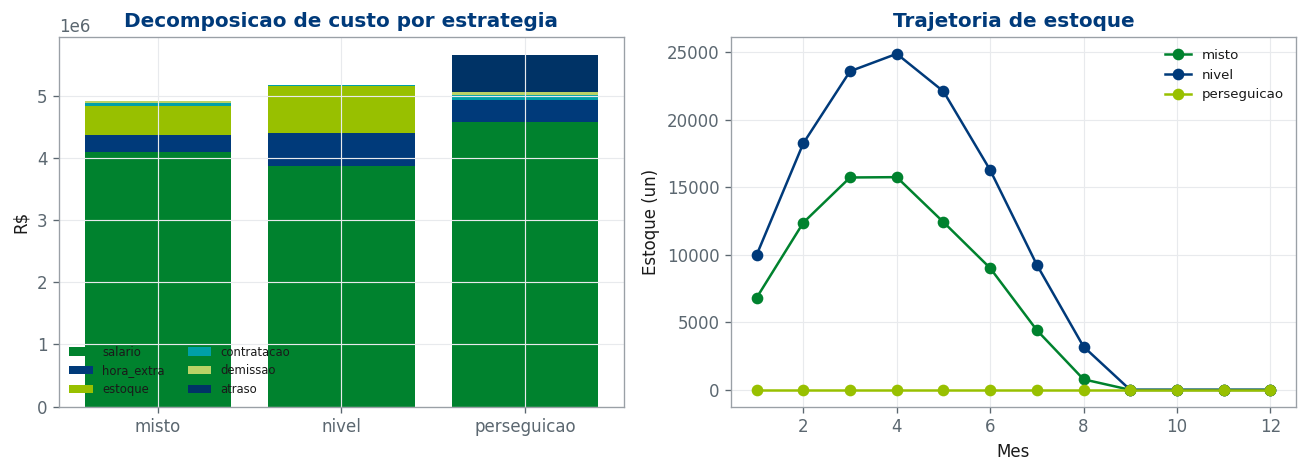
\includegraphics[keepaspectratio,alt={Figura 4 - Decomposição de custo e trajetória de estoque por estratégia.}]{figuras/fig04_cenarios.png}}
\caption{Figura 4 - Decomposição de custo e trajetória de estoque por
estratégia.}
\end{figure}

\begin{figure}
\centering
\pandocbounded{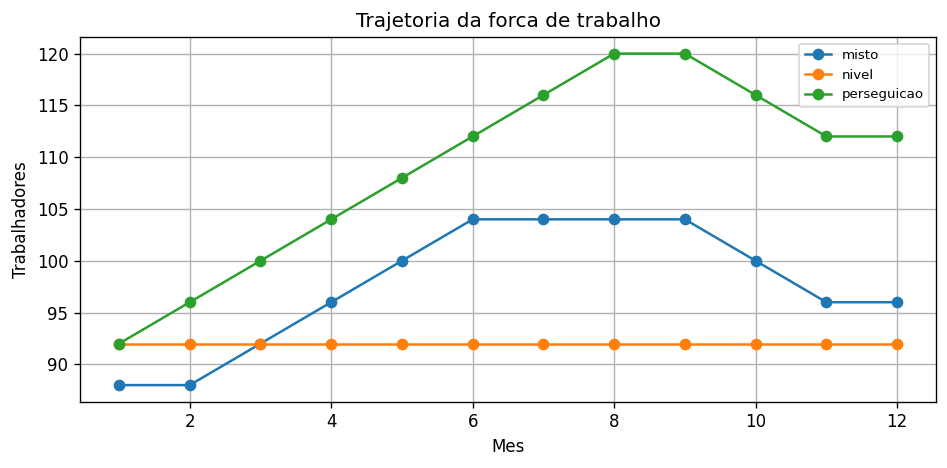
\includegraphics[keepaspectratio,alt={Figura 5 - Trajetória da força de trabalho por estratégia.}]{figuras/fig05_forca_trabalho.png}}
\caption{Figura 5 - Trajetória da força de trabalho por estratégia.}
\end{figure}

\subsubsection{6.4 Preços-sombra: onde a capacidade
vale}\label{preuxe7os-sombra-onde-a-capacidade-vale}

Os preços-sombra da restrição de capacidade regular (Figura 6) revelam
\textbf{onde e quanto vale ampliar a capacidade}. Fora da janela de
aperto (meses 1 e 10 a 12), a capacidade é ociosa e não vale nada. Na
aproximação do pico, o valor cresce de forma regular --- cerca de
\textbf{R\$ 6 por unidade a cada mês}, chegando a R\$ 48/un no mês 9. O
incremento de R\$ 6 é exatamente o custo mensal de estoque: uma unidade
de capacidade extra em um mês anterior permitiria antecipar produção e
carregá-la até o pico, e o valor dessa antecipação é o custo de estoque
evitado no caminho. Em termos gerenciais, isso diz que \textbf{ampliar
capacidade só compensa nos meses pré-pico}, e que o valor de um
trabalhador adicional (≈180 un de capacidade) nesses meses é
substancial.

\begin{figure}
\centering
\pandocbounded{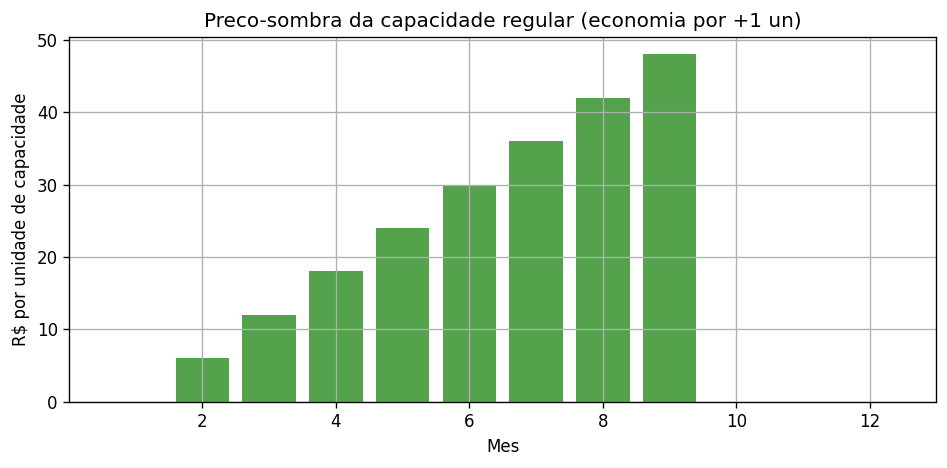
\includegraphics[keepaspectratio,alt={Figura 6 - Preço-sombra da capacidade regular por mês.}]{figuras/fig06_precos_sombra.png}}
\caption{Figura 6 - Preço-sombra da capacidade regular por mês.}
\end{figure}

\subsubsection{6.5 Sensibilidade dos
parâmetros}\label{sensibilidade-dos-paruxe2metros}

O diagrama de tornado (Figura 7) mostra a variação do custo ótimo quando
cada parâmetro é alterado em ±20\%. O custo é mais sensível ao
\textbf{nível de demanda} e ao \textbf{salário}, e comparativamente
pouco sensível a custos de contratação/demissão e atraso --- coerente
com o fato de o plano misto usar esses instrumentos com parcimônia. Essa
hierarquia orienta onde vale a pena investir em melhor informação
(previsão de demanda) e negociação (custo de mão de obra).

\begin{figure}
\centering
\pandocbounded{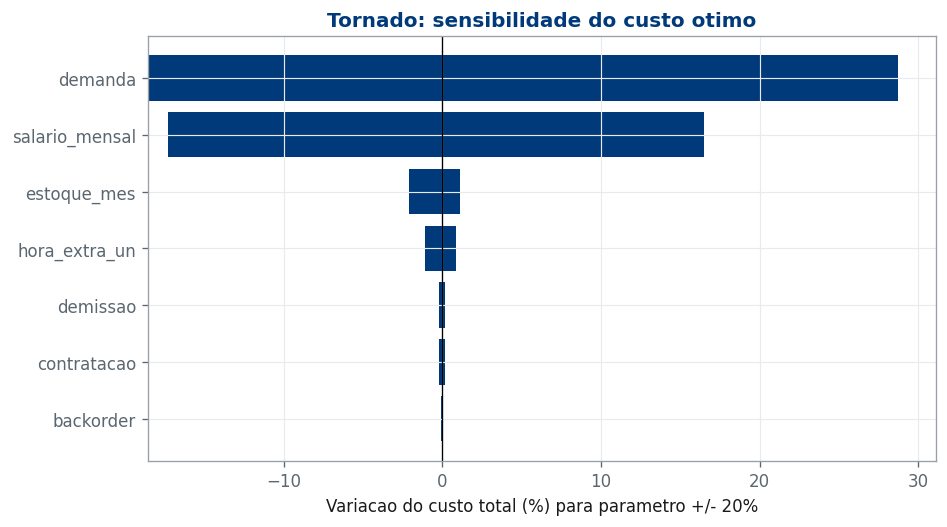
\includegraphics[keepaspectratio,alt={Figura 7 - Tornado de sensibilidade do custo ótimo.}]{figuras/fig07_tornado.png}}
\caption{Figura 7 - Tornado de sensibilidade do custo ótimo.}
\end{figure}

\subsubsection{6.6 Fronteira custo × nível de
serviço}\label{fronteira-custo-nuxedvel-de-serviuxe7o}

A Figura 8 e a Tabela 4 traçam o preço de cada ponto de serviço. Elevar
o serviço exige mais estoque de segurança, dimensionado pelo erro de
previsão medido na Seção 6.1. Sair de 80\% para 95\% custa cerca de +1,8
ponto percentual de custo; ir de 95\% para 99\% custa mais +1,6 p.p. O
joelho da curva sugere que \textbf{95\% é um alvo eficiente}: acima
disso, o custo do serviço cresce mais rápido que o benefício.

\textbf{Tabela 4 - Fronteira custo × serviço}

{\def\LTcaptype{none} % do not increment counter
\begin{longtable}[]{@{}lll@{}}
\toprule\noalign{}
Nível de serviço & Custo total (R\$) & Acréscimo vs base \\
\midrule\noalign{}
\endhead
\bottomrule\noalign{}
\endlastfoot
80\% & 5.011.742 & +2,0\% \\
90\% & 5.062.164 & +3,0\% \\
95\% & 5.103.825 & +3,8\% \\
99\% & 5.182.438 & +5,4\% \\
\end{longtable}
}

\begin{figure}
\centering
\pandocbounded{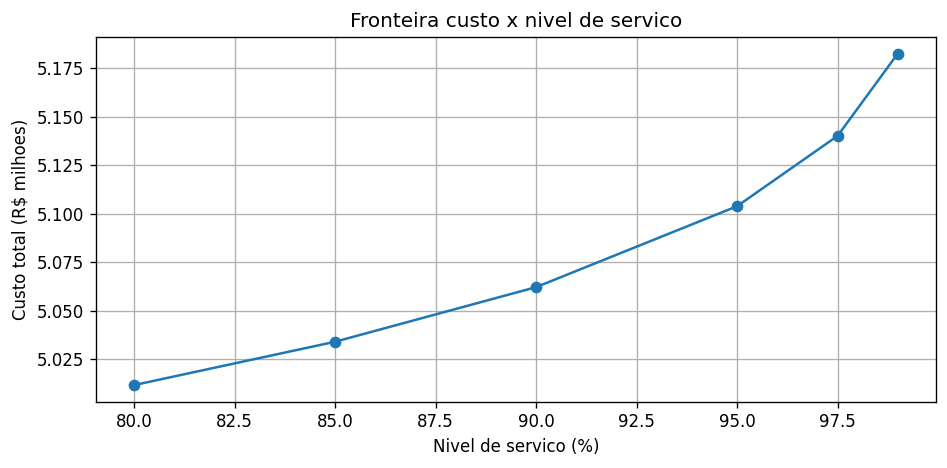
\includegraphics[keepaspectratio,alt={Figura 8 - Fronteira custo × nível de serviço.}]{figuras/fig08_fronteira.png}}
\caption{Figura 8 - Fronteira custo × nível de serviço.}
\end{figure}

\subsubsection{6.7 Robustez sob incerteza (Monte
Carlo)}\label{robustez-sob-incerteza-monte-carlo}

Por fim, testo o plano comprometido contra a incerteza: fixo a produção
do plano e simulo 2.000 realizações da demanda (previsão ± erro),
medindo custo realizado e nível de serviço (Figura 9). O plano
determinístico já é razoavelmente robusto, atingindo \textbf{serviço
médio de 98,8\%}, mas cumpre a meta de 95\% em apenas 97\% dos cenários.
Adicionar o estoque de segurança de 95\% eleva o serviço médio para
99,2\% e, mais importante, \textbf{eleva para 99\% a fração de cenários
que cumprem a meta}, a um custo adicional de cerca de 2\%. O valor do
estoque de segurança está, portanto, na \textbf{proteção de cauda}:
reduzir o risco de falhar a meta nos cenários adversos.

\begin{figure}
\centering
\pandocbounded{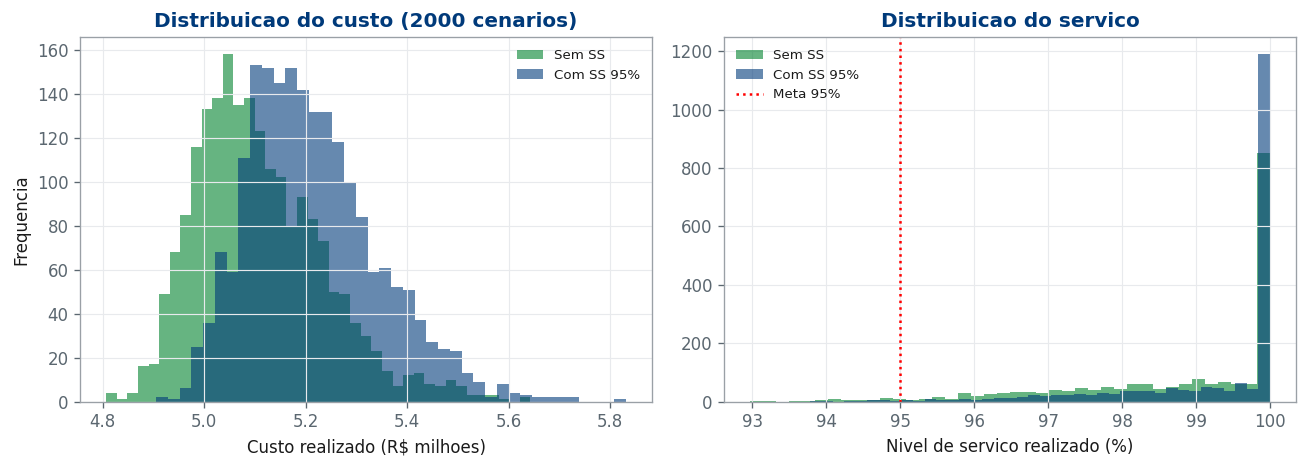
\includegraphics[keepaspectratio,alt={Figura 9 - Distribuição de custo e de nível de serviço realizados (2.000 cenários).}]{figuras/fig09_montecarlo.png}}
\caption{Figura 9 - Distribuição de custo e de nível de serviço
realizados (2.000 cenários).}
\end{figure}

\begin{center}\rule{0.5\linewidth}{0.5pt}\end{center}

\subsection{7. Tomada de decisão e
trade-offs}\label{tomada-de-decisuxe3o-e-trade-offs}

\textbf{Recomendo adotar o plano misto com estoque de segurança
calibrado para 95\% de nível de serviço.} A justificativa é quantitativa
e responde às perguntas centrais do problema:

\begin{itemize}
\tightlist
\item
  \textbf{Qual estratégia?} A mista domina as puras (nível +5,2\%,
  perseguição +15,2\%). A comparação não é óbvia a priori: exige o
  modelo para desempatar, e o modelo mostra que a resposta é combinar
  instrumentos, não usar um só.
\item
  \textbf{Onde está o gargalo?} Na capacidade dos meses pré-pico; os
  preços-sombra quantificam seu valor e indicam que antecipar produção
  em estoque é mais barato do que depender de hora extra e contratações
  no pico --- por isso o plano pré-constrói estoque.
\item
  \textbf{Quanto custa o serviço?} A fronteira mostra que 95\% é um alvo
  eficiente; subir a 99\% custa mais 1,6 p.p. de custo.
\item
  \textbf{O plano é robusto?} Sim; e o estoque de segurança compra
  proteção de cauda (cobertura da meta de 97\% para 99\% dos cenários)
  por \textasciitilde2\% de custo.
\end{itemize}

Os principais \textbf{trade-offs} avaliados são: custo total × nível de
serviço (fronteira); estabilidade da força de trabalho × custo de
estoque (nível vs perseguição); e flexibilidade de curto prazo × custo
de antecipação (hora extra vs estoque).

\textbf{Riscos e limitações.} O modelo assume custos determinísticos e
um único produto agregado; o lead time é implícito e fixo. Extensões
naturais e de alto valor seriam: (i) lead time de fornecimento
estocástico; (ii) desagregação do plano em um Programa Mestre de
Produção (MPS) e MRP multiproduto; e (iii) uma formulação
estocástica/robusta em dois estágios, em vez do plano determinístico com
Monte Carlo \emph{ex post}. Ainda assim, para a decisão agregada de 12
meses, a abordagem adotada é adequada e conservadora.

\begin{center}\rule{0.5\linewidth}{0.5pt}\end{center}

\subsection{8. Conclusão}\label{conclusuxe3o}

Transformei um problema de PCP em uma decisão fundamentada em evidência
quantitativa. Partindo de uma previsão de demanda validada (SARIMA, MAPE
5,4\%), formulei e resolvi o planejamento agregado por programação
linear, comparei estratégias, extraí preços-sombra, tracei a fronteira
custo × serviço e testei a robustez por simulação. O plano misto com
estoque de segurança de 95\% é a política recomendada: minimiza o custo
total relevante (R\$ 4,92 milhões), domina as estratégias puras e mantém
o nível de serviço sob incerteza a um custo marginal pequeno.

A principal implicação para o PCP é que o valor do planejamento agregado
não está em nenhum instrumento isolado --- estoque, força de trabalho ou
hora extra ---, mas em \textbf{coordená-los} ao longo do tempo em função
da sazonalidade e da incerteza. Como possíveis extensões, destaco a
integração com MPS/MRP, a modelagem de lead time estocástico e a
otimização robusta, que aprofundariam a decisão sem alterar sua
estrutura central.

\begin{center}\rule{0.5\linewidth}{0.5pt}\end{center}

\subsection{Referências}\label{referuxeancias}

CHOPRA, S.; MEINDL, P. \emph{Supply Chain Management: Strategy,
Planning, and Operation}. Pearson Education. (fundamentos de estoque e
nível de serviço.)

HOPP, W. J.; SPEARMAN, M. L. \emph{Factory Physics}. Waveland Press.
(dinâmica de sistemas produtivos, variabilidade, Lei de Little.)

NAHMIAS, S.; OLSEN, T. L. \emph{Production and Operations Analysis}.
Waveland Press. (planejamento agregado, previsão de demanda e gestão de
estoques.)

\end{document}
